
%% gnuplot の test

\documentclass[10pt,b5paper,papersize,dvipdfmx]{jsbook}

\usepackage{../../../sty/vuccaken}
% \usepackage[analog]{vuccaken}
% \usepackage{v-hyperref}
\usepackage{../../../sty/vuccaken2019}

\usepackage{newtxtext,newtxmath}

%% font -> gt & sf
\renewcommand\kanjifamilydefault{\gtdefault}
\renewcommand\familydefault{\sfdefault}


\usepackage{gnuplot-lua-tikz}

%
\begin{document}
%

\begin{figure}[th] \small
  \centering
  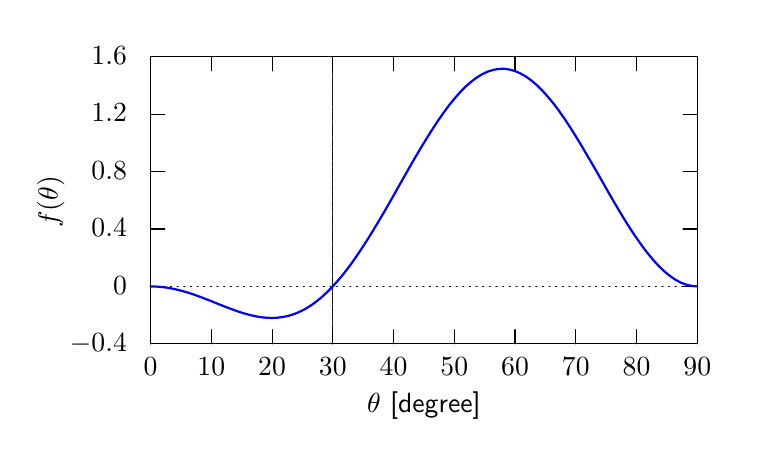
\begin{tikzpicture}[gnuplot]
%% generated with GNUPLOT 5.1p0 (Lua 5.3; terminal rev. 99, script rev. 100)
%% 土 11/23 01:34:26 2019
\path (0.000,0.000) rectangle (9.000,5.000);
\gpcolor{color=gp lt color border}
\gpsetlinetype{gp lt border}
\gpsetdashtype{gp dt solid}
\gpsetlinewidth{1.00}
\draw[gp path] (1.504,0.985)--(1.684,0.985);
\draw[gp path] (8.447,0.985)--(8.267,0.985);
\node[gp node right] at (1.320,0.985) {$-0.4$};
\draw[gp path] (1.504,1.714)--(1.684,1.714);
\draw[gp path] (8.447,1.714)--(8.267,1.714);
\node[gp node right] at (1.320,1.714) {$0$};
\draw[gp path] (1.504,2.443)--(1.684,2.443);
\draw[gp path] (8.447,2.443)--(8.267,2.443);
\node[gp node right] at (1.320,2.443) {$0.4$};
\draw[gp path] (1.504,3.173)--(1.684,3.173);
\draw[gp path] (8.447,3.173)--(8.267,3.173);
\node[gp node right] at (1.320,3.173) {$0.8$};
\draw[gp path] (1.504,3.902)--(1.684,3.902);
\draw[gp path] (8.447,3.902)--(8.267,3.902);
\node[gp node right] at (1.320,3.902) {$1.2$};
\draw[gp path] (1.504,4.631)--(1.684,4.631);
\draw[gp path] (8.447,4.631)--(8.267,4.631);
\node[gp node right] at (1.320,4.631) {$1.6$};
\draw[gp path] (1.504,0.985)--(1.504,1.165);
\draw[gp path] (1.504,4.631)--(1.504,4.451);
\node[gp node center] at (1.504,0.677) {$0$};
\draw[gp path] (2.275,0.985)--(2.275,1.165);
\draw[gp path] (2.275,4.631)--(2.275,4.451);
\node[gp node center] at (2.275,0.677) {$10$};
\draw[gp path] (3.047,0.985)--(3.047,1.165);
\draw[gp path] (3.047,4.631)--(3.047,4.451);
\node[gp node center] at (3.047,0.677) {$20$};
\draw[gp path] (3.818,0.985)--(3.818,1.165);
\draw[gp path] (3.818,4.631)--(3.818,4.451);
\node[gp node center] at (3.818,0.677) {$30$};
\draw[gp path] (4.590,0.985)--(4.590,1.165);
\draw[gp path] (4.590,4.631)--(4.590,4.451);
\node[gp node center] at (4.590,0.677) {$40$};
\draw[gp path] (5.361,0.985)--(5.361,1.165);
\draw[gp path] (5.361,4.631)--(5.361,4.451);
\node[gp node center] at (5.361,0.677) {$50$};
\draw[gp path] (6.133,0.985)--(6.133,1.165);
\draw[gp path] (6.133,4.631)--(6.133,4.451);
\node[gp node center] at (6.133,0.677) {$60$};
\draw[gp path] (6.904,0.985)--(6.904,1.165);
\draw[gp path] (6.904,4.631)--(6.904,4.451);
\node[gp node center] at (6.904,0.677) {$70$};
\draw[gp path] (7.676,0.985)--(7.676,1.165);
\draw[gp path] (7.676,4.631)--(7.676,4.451);
\node[gp node center] at (7.676,0.677) {$80$};
\draw[gp path] (8.447,0.985)--(8.447,1.165);
\draw[gp path] (8.447,4.631)--(8.447,4.451);
\node[gp node center] at (8.447,0.677) {$90$};
\gpsetlinetype{gp lt axes}
\gpsetdashtype{gp dt axes}
\draw[gp path] (1.504,1.714)--(8.447,1.714);
\draw[gp path] (1.504,0.985)--(1.504,4.631);
\gpsetlinetype{gp lt border}
\gpsetdashtype{gp dt solid}
\draw[gp path] (1.504,4.631)--(1.504,0.985)--(8.447,0.985)--(8.447,4.631)--cycle;
\gpsetdashtype{dash pattern=on 1.00*\gpdashlength off 1.00*\gpdashlength }
\draw[gp path](3.818,0.985)--(3.818,4.631);
\node[gp node center,rotate=-270] at (0.246,2.808) {$f(\theta)$};
\node[gp node center] at (4.975,0.215) {$\theta$ [degree]};
\gpcolor{rgb color={0.000,0.000,1.000}}
\gpsetdashtype{gp dt solid}
\gpsetlinewidth{2.00}
\draw[gp path] (1.504,1.714)--(1.574,1.712)--(1.644,1.707)--(1.714,1.698)--(1.785,1.685)%
  --(1.855,1.670)--(1.925,1.651)--(1.995,1.630)--(2.065,1.607)--(2.135,1.581)--(2.205,1.554)%
  --(2.275,1.527)--(2.346,1.498)--(2.416,1.470)--(2.486,1.443)--(2.556,1.417)--(2.626,1.392)%
  --(2.696,1.370)--(2.766,1.351)--(2.836,1.335)--(2.907,1.323)--(2.977,1.316)--(3.047,1.313)%
  --(3.117,1.317)--(3.187,1.326)--(3.257,1.341)--(3.327,1.363)--(3.398,1.392)--(3.468,1.427)%
  --(3.538,1.470)--(3.608,1.521)--(3.678,1.578)--(3.748,1.643)--(3.818,1.714)--(3.888,1.793)%
  --(3.959,1.878)--(4.029,1.969)--(4.099,2.067)--(4.169,2.170)--(4.239,2.277)--(4.309,2.389)%
  --(4.379,2.505)--(4.450,2.624)--(4.520,2.745)--(4.590,2.868)--(4.660,2.992)--(4.730,3.116)%
  --(4.800,3.239)--(4.870,3.360)--(4.940,3.479)--(5.011,3.595)--(5.081,3.706)--(5.151,3.813)%
  --(5.221,3.914)--(5.291,4.009)--(5.361,4.096)--(5.431,4.176)--(5.501,4.248)--(5.572,4.310)%
  --(5.642,4.364)--(5.712,4.407)--(5.782,4.440)--(5.852,4.463)--(5.922,4.476)--(5.992,4.478)%
  --(6.063,4.468)--(6.133,4.449)--(6.203,4.418)--(6.273,4.378)--(6.343,4.327)--(6.413,4.267)%
  --(6.483,4.197)--(6.553,4.119)--(6.624,4.033)--(6.694,3.939)--(6.764,3.839)--(6.834,3.733)%
  --(6.904,3.621)--(6.974,3.506)--(7.044,3.387)--(7.115,3.266)--(7.185,3.144)--(7.255,3.021)%
  --(7.325,2.898)--(7.395,2.777)--(7.465,2.659)--(7.535,2.544)--(7.605,2.434)--(7.676,2.328)%
  --(7.746,2.229)--(7.816,2.137)--(7.886,2.052)--(7.956,1.975)--(8.026,1.908)--(8.096,1.850)%
  --(8.166,1.801)--(8.237,1.763)--(8.307,1.736)--(8.377,1.720)--(8.447,1.714);
\gpcolor{color=gp lt color border}
\gpsetlinewidth{1.00}
\draw[gp path] (1.504,4.631)--(1.504,0.985)--(8.447,0.985)--(8.447,4.631)--cycle;
%% coordinates of the plot area
\gpdefrectangularnode{gp plot 1}{\pgfpoint{1.504cm}{0.985cm}}{\pgfpoint{8.447cm}{4.631cm}}
\end{tikzpicture}
%% gnuplot variables

  \caption{$f(\theta) = \cos^2 3\theta + \sin^2 2\theta - \cos^2\theta$のプロット.$0 < \theta < 30^\circ$のとき$f(\theta) < 0$である.}
  \label{a}
\end{figure}











%
%%
%%%
%%%%
%%%%%
%%%%%%
%%%%%%%
%%%%%%%%
%%%%%%%%%
%%%%%%%%%%
%%%%%%%%%%%
%%%%%%%%%%%%
%%%%%%%%%%%%%
\end{document}
%%%%%%%%%%%%%
%%%%%%%%%%%%
%%%%%%%%%%%
%%%%%%%%%%
%%%%%%%%%
%%%%%%%%
%%%%%%%
%%%%%%
%%%%%
%%%%
%%%
%%
%